\documentclass[doc,a4paper,12pt]{apa6}
\usepackage[utf8]{inputenc}
\usepackage[T1]{fontenc}
\usepackage[ngerman]{babel}
\usepackage{amsmath}
\usepackage[doublespacing]{setspace}
\usepackage{paralist}
\usepackage{graphicx}
\usepackage{epstopdf}
\usepackage{wrapfig}
\usepackage{float}
\usepackage{csquotes}
\usepackage[backend=biber,style=apa]{biblatex}
\DeclareLanguageMapping{ngerman}{ngerman-apa}
\DefineBibliographyStrings{ngerman}{andothers={et\ al\adddot}} 

\bibliography{references}
 
\title{Explizite Detektion von Abweichungen in komplexen Regeln bei auditiven Stimuli}
\shorttitle{Explizite Komplexe Regelerkennung}
\author{Carlo Michaelis}
\date{23. August 2013}
\affiliation{Universität Leipzig}
\abstract{Abstract}
\ccoppy{Creative Commons (CC BY 3.0)}

\setlength{\skip\footins}{1.5em}
\setlength{\footnotesep}{1.5em}
\setlength{\textfloatsep}{2em}
\raggedbottom
\begin{document}

%\maketitle
%\newpage

%\tableofcontents
%\newpage

\section{Einleitung}

Viele Fragen sind bis heute ungeklärt und werden es wohl auch weiterhin bleiben. Trotzdem scheint es, als gäbe es – vor allem bei der Erklärung unserer physikalischen Umgebung – schon einige befriedigende Antworten, die nicht nur die notwendige Funktionalität ermöglichen, sondern Großteils bereits unseren Hunger nach Verständnis decken. In einem Bereich jedoch, dem Bereich psychischer Prozesse, gibt es zwar bereits viele Einzelerkenntnisse, eine umfassende Theorie über die psychischen Funktionsweisen komplexerer Organismen steht jedoch aus. Vor allem das Zusammenspiel, also die Schnittstelle zwischen der Psyche und dem Körper, die Frage nach Determiniertheit und Selbstbestimmung, nach automatischer und willentlicher Verarbeitung sind bei weitem noch nicht ganzheitlich geklärt.\\
Dabei erfüllt das Verständnis darüber nicht nur den Zweck Wissen über Lebewesen zu akkumulieren oder einige neugierige Personen zu befriedigen, vielmehr prägt die Erkenntnis über die Funktionsweise unsere Gesellschaft, sie entscheidet u.a. über Gesetze, Konventionen und Kultur.\\
So sehr wir uns als Menschen auch immer wieder selbstverständlich einen freien Willen unterstellen und damit die Fähigkeit durch den Geist gezielt und indeterminiert unsere Welt verändern zu können, ohne unwillkürlich automatisch ablaufende Verhaltensweisen wäre ein Leben auf der Erde wohl unmöglich. In vielen Situationen müssen innerhalb kürzester Zeit bestehende Reize erfasst, zukünftige Ereignisse simuliert und schließlich vorhergesagt werden.

Ein gutes Beispiel für die hohe Leistungsfähigkeit der automatisch ablaufenden Systeme des Menschen ist seine Sprache. Deutlich wird dies schon allein durch das Segmentationsproblem des Sprachverstehens. Mit physikalischen Mitteln aufgezeichnete Frequenzen von Schallwellen zeigen Muster, die bei visueller Betrachtung kaum korrekt in Worte getrennt werden können. Eine Pause oder eine Frequenzschwankung sagt nur selten tatsächlich auch den Beginn eines neuen Wortes vorher. Zur Segmentation der Worte werden bei weitem nicht nur die physikalischen Signale, sondern zusätzlich viele verschiedene Hinweisreize benötigt \parencites[u.a.][]{brent1996distributional}{saffran1996word}. Wichtig sind vor allem Lautfolgen, die in verschiedenen Sprachen nur mit einer bestimmten Wahrscheinlichkeit oder sogar gar nicht vorkommen. Die Folge von "x" und "s" würde in der Deutschen Sprache nicht erwartet werden und liefert dem auditiven System keine semantische Information. Das System wurde in diesem Fall zum Beispiel eher von zwei Wörtern ausgehen. Eines, das auf "x" endet, und eines, das mit "s" beginnt (z.B. "Max sieht"). Dabei muss die Segmentation nicht nur anhand einer großen Menge an Informationen, sondern auch innerhalb kürzester Zeit erfolgen, die ohne eine automatisierte Verarbeitung wohl kaum möglich wäre.\\
Beim Sprechen wiederum ist zum Beispiel das so genannte Speech Monitoring \parencites{levelt1983monitoring}{postma2000detection} von hoher Bedeutung. Das bezeichnet die Fähigkeit die inhaltliche Qualität des gesprochenen noch während dem Sprechen reflektieren zu können. Das wiederum bedeutet, dass beim Sprechen mindestens zwei Prozesse gleichzeitig statt finden. Das legt nah, dass hier ein hoher Grad an automatischer Verarbeitung im Spiel ist. In einer Studie von \textcite{goldman1958speech} konnte gezeigt werden, dass u.a. immer dann größere Sprechpausen entstehen, wenn kommende Wörter schwerer vorhersagbar sind. Der automatischer Verarbeitungsprozess der Vorhersage scheint also nicht unbegrenzt effizient zu sein, auch die automatischen Prozesse sind augenscheinlich Abhängig von der der Komplexität der Aufgabe.\\
Bezüglich der auditiven Komponente sei vor allem auch die Musik hervorgehoben. Gerade in der Musik spiegelt sich die Tendenz des Menschen zu erfolgreichen automatischen Vorhersagen wider. \textcite{drake2001quest} prüften 5 universelle, d.h. nicht-kulturabhängige Paradigmen, wie sich Menschen zu Musik verhalten. In Paradigma 3 beschrieben sie, dass sich Menschen, die im Takt der Musik bleiben sollen, in mehr als 90\% der Zeit erfolgreich mit Musik synchronisieren können. D.h. Vorhersagen können erfolgreich getroffen und Handlungen entsprechend erfolgreich an den Vorhersagen ausgerichtet werden. Ein Verhalten, dass auch bei unmusikalischen Menschen auftritt und damit auch hier einen Hinweis für ein automatisches Verhalten liefert. Man könnte mutmaßen, dass genau in der Vorhersagbarkeit, die anscheinend mehr passiv mit dem Menschen geschieht, als dass diese aktiv hervorgerufen wird, der Reiz der Musik liegt und auch ein Harmonieempfinden damit zusammenhängt.

%"Max sieht" -> Nicht Silbengrenze, sondern Wortgrenze, vereinfachtes Beispiel

Die Bedeutung der Vorhersagbarkeit und vor allem der diesbezüglich wirkenden automatischen Verarbeitung lässt sich an den vorigen Beispielen recht gut erkennen. Im folgenden Experiment soll es um die Vorhersagbarkeit von komplexen Regeln in auditiven Stimuli gehen. Konkret soll untersucht werden inwiefern komplexe Regeln von Tonabfolgen (wie sie etwa auch in der Sprache vorkommen) erkannt und insbesondere vorhergesagt bzw. Abweichungen erkannt werden können. Im Folgenden soll zunächst der Forschungsstand bezüglich der auditiven Regelerkennung und der Vorhersagefähigkeit erläutert werden. Anschließend wird eine kurze Einführung in Lerntheorien erfolgen, die speziell für dieses Experiment von Bedeutung sein wird. Und zuletzt soll in der Diskussion und der folgenden Post-Hoc-Analyse versucht werden die genannten Beispiele einzuordnen.

\subsection{Mismatch Negativity (MMN) und das Oddball Paradigma}

Die Mismatch Negativity (MMN) ist ein ereigniskorreliertes Potential (EKP). Bei ereigniskorrelierten Potentialen handelt es sich um elektrische Potentiale des Gehirns, welche zu einem bestimmten Zeitpunkt (Ereignis) eintreten und mit diesem zusammenhängen und daher als ereigniskorreliert betrachtet werden können. Die Messung dieser Signale erfolgt per Elektroenzephalogramm (EEG), welches elektrische Potentiale des Gehirns erfassen kann. Um die Signale, welche durch das Ereignis ausgelöst werden, letztlich vom Rauschen anderer Gehirnpotentiale trennen zu können, werden die Potentiale über mehrere Messungen gemittelt.

Erstmals wurde die MMN von \textcite{naatanen1978early} für auditive Stimuli beschrieben. Verwendet wurde das so genannte Oddball Paradigma, bei dem eine Reihe gleicher Stimuli gegeben wird, welche dann von einem nicht-regelkonformen Stimulus unterbrochen wird. Die MMN trifft dann ca. 150ms – 250ms nach der Präsentation des Abweichers vor allem im fronto-zentralen Bereich auf. Sie zeigt damit an, dass eine Vorhersage (bzw. eine Extrapolation) des Gehirns fehlerhaft war. Im Umkehrschluss lässt sich bei einem Auftreten der MMN schließen, dass das Gehirn zuvor eine Regelmäßigkeit erkannt haben muss \parencite{schroger2007mismatch}. Auf dieser Logik basieren auch die Studien, die diesem Experiment zugrunde liegen.

Eine weitere Eigenschaft der MMN ist, dass sie auch dann auftritt, wenn der auditive Stimulus nicht beachtet wird \parencite{naatanen2007mismatch}, zum Beispiel wenn Probanden während des Hörens der Töne einen Stummfilm schauen. Das Gehirn scheint also keine oder nur sehr wenige Aufmerksamkeitsressourcen für die Erkennung einer Regelmäßigkeit in einem auditiven Stimulus zu benötigen. Die Verarbeitung erfolgt damit folglich automatisiert.

\subsection{Komplexe Regelerkennung}

Es stellte sich schon bald die Frage, ob die MMN auch bei deutlich komplexeren Regeln auftritt. Dies würde implizieren, dass das Gehirn die Fähigkeit besitzt, auch komplexe Regeln zu extrahieren und vorhersagen zu können.\\
Bereits in früheren Studien wurden Paradigmen für komplexe Regeln entwickelt. Diese verwendeten zwar nicht das Konzept der MMN, konnten aber bereits nachweisen, dass die Probanden die Regeln nicht bewusst erkennen können. Im Sequence Learning Paradigm \parencite{hoffmann1998implicit} sollten die Probanden ein sich wiederholendes Muster erkennen, welches in einer Ton-Sequenz versteckt war, im Covariation Detection Paradigm \parencite{stamov2001revealing}, wiederum lernten die Probanden nichtsaliente Verbindungen zwischen den einzelnen Stimulus-Elementen. Obwohl die Probanden die Regeln meist nicht bewusst erkannten, zeigten sich durch Übung Leistungssteigerungen in Form von zunehmend erhöhter Geschwindigkeit und erhöhter Genauigkeit, was zunächst auf implizites Lernen hinweist.

\textcite{paavilainen2007preattentive} warfen daraufhin die Frage auf in welchem Ausmaß der Erkennungsprozess Aufmerksamkeitsressourcen benötigt. Dabei sollte vor allem geklärt werden, ob die Erkennung komplexerer Regeln bereits präattentiv auf der Ebene des sensorischen Gedächtnisses stattfindet. Um dies zu untersuchen wurden den Probanden Töne vorgespielt, die sich in ihrer Länge (50ms oder 150ms) und in ihrer Höhe (1000Hz oder 1500Hz) unterschieden. Allgemein wurden für die Tonfolgen zwei Regeln verwendet.

\begin{compactitem}
  \item Auf einen langen Ton folgt ein hoher Ton, auf einen kurzen Ton folgt ein tiefer
Ton
  \item Auf einen langen Ton folgt ein tiefer Ton, auf einen kurzen Ton folgt ein hoher
Ton
\end{compactitem}

\begin{figure}[t]
  \centering
  \begin{minipage}{\textwidth}
    \setlength{\fboxsep}{.05\textwidth}
    \fbox{\begin{minipage}{.9\textwidth}
      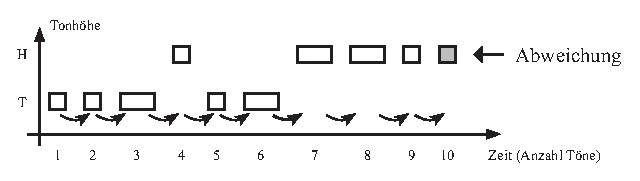
\includegraphics[width=\textwidth]{abb2-tones.eps}
    \end{minipage}}
    \vspace{10pt}
    \caption{Beispiel für eine Tonsequenz. Die Länge des einen Tons sagt die Höhe des nächsten Tons vorher. In diesem Beispiel folgt auf einen kurzen Ton ein tiefer Ton und auf einen langen Ton ein hoher Ton. Der letzte Ton ist im Beispiel von der Regel abweichend. Auf einen kurzen Ton (Ton 9) folgt kein tiefer Ton, wie die Regel es vorhersagen würde, sondern ein hoher Ton (Ton10).}
    \label{stimuli}
  \end{minipage}
\end{figure}

Von den zwei Merkmalen (Höhe und Länge) ist dem Prinzip nach jeweils die Länge der entscheidende Prädiktor für das Merkmal Höhe des nächsten Tons. Während dem Versuch bekam die eine Hälfte der Probanden die eine Regel, die anderen Hälfte die andere Regel präsentiert. Um die MMN auszulösen wurde die Regel an vereinzelten Stellen unterbrochen. Eine Beispielsequenz dieser Regel ist in Abbildung \ref{stimuli} gezeigt.\\
Alle Probanden durchliefen in gegebener Reihenfolge außerdem folgende Bedingungen:

\begin{compactitem}
  \item \textbf{Ignore}: Die Probanden schauten einen Stummfilm mit Untertiteln und sollten weder auf die Töne achten, noch darauf reagieren.
  \item \textbf{Implicit detection}: Den Probanden wurde die Regel nicht erklärt, sie sollten jedoch eine Taste drücken wenn sie das Gefühl hätten, dass ein Ton nicht passt.
  \item \textbf{Explicit detection}: Den Probanden wurde die Regel erklärt (mit Hilfe eines Schaubildes), sie sollten eine Taste drücken, wenn sie der Meinung waren, dass einer der Töne nicht in die Regel passt.
\end{compactitem}

Im Ergebnis zeigte sich, dass in allen drei Bedingungen ein signifikanter Ausschlag der MMN vorlag, sofern ein Abweicher vorkam. Es zeigte sich allerdings auch, dass sich der Ausschlag der MMN in den drei Bedingungen nicht signifikant voneinander unterschied. Es war also unerheblich, ob die Probanden die Töne ignorierten, intuitiv darauf reagierten oder aktiv und bewusst darauf achteten. Eine intuitive oder bewusste Übung konnte die Erkennungsleistung des Gehirns nicht steigern. Demzufolge waren implizite, so wie explizite Lernprozesse auf Ebene der neuronalen Signale anscheinend nicht vorhanden. Für einen - zumindest kleinen - Lerneffekt spricht hingegen, dass die behavioralen Daten in den zwei detection-Bedingunen in Form der Erfolgsrate beim Drücken der Tasten signifikant vom Zufall abwichen, wenn auch nur sehr gering. Qualitativ wurde außerdem berichtet, dass die Probanden das Wissen über die Regel nur als wenig hilfreich einschätzten.\\
Aus den Ergebnissen haben \textcite{paavilainen2007preattentive} geschlossen, dass die Verarbeitung wohl überwiegend automatisiert und die Treffer in der explicit detection Bedingung eher auf Intuition, als auf explizites Wissen über die Regel zurückzuführen sind. Allerdings scheint sich die  Leistungsfähigkeit geringfügig verbessern zu können. Dies schlägt sich zumindest in der knapp überzufälligen behavioralen Erfolgsrate nieder. Letztlich war ein weiteres EKP, die so genannte P3, nicht ausgeprägt. Diese Komponente schlägt üblicherweise aus, wenn Stimuli bewusst klassifiziert werden. Die These, dass die Stimuli automatisiert und unbewusst verarbeitet werden konnte damit bestätigt werden.

Die Studie von \textcite{paavilainen2007preattentive} wurde 2 Jahre später von \textcite{bendixen2008rapid} repliziert und erweitert. Dabei wurden die gleichen Regeln verwendet, auch Tonhöhe und Frequenz entsprach den vorigen.\\
Die Regeln wurden in unterschiedlich langen Sequenzen (4, 9, 14, 19 Töne) regelkonform präsentiert und anschließend durch irreguläre Sequenzen (4-8 Töne) unterbrochen. Diese Unterbrechung führt dazu, dass das Gehirn immer wieder von vorne beginnen muss eine Regel zu erkennen, zumal nach einer irregulären Sequenz auch die reguläre Sequenz variieren kann, da wie oben beschrieben, zwei solcher regulären Regeln existieren. Es wurde zwischen zwei Bedingungen unterschieden:

%Tonanzahl nicht mehr doppelt exlizit erwähnt, aber einmal wollte ich noch, damit man eine Vorstellung davon hat wie lang solche Sequenzen sein können. Gleiches bei Blöcken unten (siehe Kommentar)

\begin{compactitem}
  \item \textbf{Passiv}: Kontinuierliche Stimuli-Präsentation, wobei die Probanden einen Stummfilm schauten und die Stimuli ignorieren sollten.
  \item \textbf{Aktiv}: Probanden hörten abgegrenzte Sequenzen unterschiedlicher Länge, wobei der letzte Ton Standard oder Deviant sein konnte. Sie bekamen die Regeln erklärt und sollten per Tastendruck reagieren.
\end{compactitem}

Die Probanden bekamen erst 8 Blöcke in der Passiv-Bedingung präsentiert, wurden gefragt, ob sie eine Regel erkannten, anschließend bekamen sie 5 weitere Blöcke in der Aktiv-Bedingung präsentiert. In keinem Fall erkannten die Probanden die Regel nach der Passiv-Bedingung korrekt, sofern sie überhaupt eine erkannten. Der Sensitivitätsindex (d-prime) lag noch signifikant über dem Zufallsniveau, sowohl für kurze (5 und 10 Töne), als auch für lange (15 und 20 Töne) Sequenzen. Die MMN zeigte jedoch nur für lange Sequenzen eine signifikante Ausprägung.\\
Die Ergebnisse von \textcite{paavilainen2007preattentive} konnten damit zum einen bestätigt werden, zum anderen konnte gezeigt werden, dass für die Regelerkennung zunächst einige Stimuli nötig sind, bis das Gehirn die entsprechende Regel abgeleitet hat. Allgemein liegt ein kontinuierlicher Zusammenhang vor. Je mehr regelkonforme Stimuli zuvor präsentiert werden, desto höher ist der Ausschlag der MMN bei einer Unterbrechung. Es scheint also eine Akkumulation abzulaufen, die Hinweise auf eine Regel ansammelt. Entscheidend ist jedoch, dass auch in dieser Studie das bewusste Erkennen einer Regelverletzung nicht möglich war. Auch hier zeigte sich die Abwesenheit der P3-Komponente und damit die Abwesenheit bewusster Klassifikationsprozesse.

\subsection{Lernen prozeduralen Wissens}

Zusammenfassend liegt also bezüglich der Erkennung komplexer Regeln eine automatisierte und unbewusste Verarbeitung vor. Während auf neuronaler Ebene Abweicher von der Regeln zuverlässig erkennt, ist es dem Mensch nicht möglich diese Regeln bewusst anzuwenden bzw. Regelabweichungen erkennen zu können. Da Lernen - kurz gefasst - als eine relativ stabile Veränderung des Verhaltens, Denkens oder Fühlens definiert wird, kann davon ausgegangen werden, dass ein Lernprozess an dieser Stelle nicht stattfindet. Eine Verhaltensbeobachtung konnte nicht oder nur in sehr geringem Maße beobachtet werden. Für eine weitere Untersuchung ist es demnach zunächst von Bedeutung zu betrachten wie das implizite und explizite prozedurale Lernen funktioniert. Daraus könnte abgeleitet werden wie ein expliziter prozeduraler Lernprozess komplexer Regeln gestaltet werden könnte. Ziel ist es einen solchen Lernprozess zu gestalten, um zu zeigen, dass ein explizites Lernen prinzipiell möglich ist. Sollte dieser Nachweis erfolgreich verlaufen, könnte dies ein Ansatz sein um die Funktionsmechanismen hinter der Lücke zwischen der automatisierten unbewussten und der manuellen bewussten Verarbeitung zu verstehen.

%Prozedural ist hier wichtig, weil angewandte Modelle darauf basieren. Wird in Dikussion allerdings dann kritisch betrachtet.

Grundsätzlich lässt sich der Lernprozess als prozedurales Lernen (abgegrenzt von deklarativem Lernen) klassifizieren, sofern das Drücken der Taste passend zu den Abweichern gelernt wird. Das Lernen deklarativen Wissens würde voraussetzen, dass es für die Erkennung reichen würde das Wissen über die Regel zu kennen. Wie sich bisher gezeigt hat, scheint das reine Wissen jedoch nicht ausreichend zu sein. Das erworbene Wissen muss bei der Erkennung von Abweichungen auf einen Handlungsprozess umgewandelt werden. Das prozedurale Lernen bezieht sich dabei weniger auf das Ausführen sichtbarer Handlungen, sondern vielmehr auf das Lernen einer Abfolge unterschiedlicher Verarbeitungsschritte.\\
In den bisherigen Untersuchungen lag – wenn überhaupt – nur implizites Lernen vor. Interessant wäre also zu betrachten wie explizites Lernen erreicht werden kann, welches bisher den Probanden nicht möglich war. Es ist auf Grund der genannten Ergebnisse davon auszugehen, dass sich ein expliziter Lernprozess relativ schwierig gestalten könnte.

Die Klassifikation in prozedurale Prozesse macht nun deutlich, dass ein einfaches Zeigen der Regel (z.B. an einem Schaubild) kaum ausreichen kann, um die Regel adäquat anzuwenden, zumal die Stimuli mit 50ms bzw. 150ms Länge und einem Inter-Stimulus-Intervall (ISI) von 300ms präsentiert wurden. Diese hohe Geschwindigkeit erfordert wahrscheinlich ein langes Training, sofern ein expliziter Prozess verlangt wird. \textcite{fitts1967human} gingen davon aus, dass prozedurales Wissen über drei Schritte hintereinander gelernt werden kann:

\begin{compactenum}
  \item \textbf{Kognitives Stadium}: In diesem Stadium handelt es sich noch um eine deklarative Repräsentation. Das deklarative Wissen kann in bestehendes Wissen integriert und mit diesem verknüpft werden. Eine Vermittlung sollte präzise und verständlich erfolgen. Angewendet werden kann z.B. ein Schaubild.
  \item \textbf{Assoziatives Stadium}: Eine prozedurale Repräsentation wird aufgebaut. Es entwickeln sich Wenn-Dann-Regeln. Sofern ein bestimmtes Ereignis eintritt wird automatisch eine spezifische Reaktion ausgeführt. Dieses Stadium kann vor allem durch regelmäßige Übung erreicht werden. Wichtig ist hier auch das Geben von Feedback.
  \item \textbf{Autonomes Stadium}: Das prozedurale Wissen kann schnell und automatisiert abgerufen werden. Die einzelnen Repräsentationen sind stabil miteinander verbunden und führen zu einer fehlerfreien Ausführung. Der Ressourcenaufwand minimiert sich. Erreicht wird dies durch das Praktizieren über längere Zeiträume.
\end{compactenum}

Eine gute Beschreibung des prozeduralen Lernens bietet auch der Learning Cycle von \textcite{whitmore2009coaching}. Der Kreislauf teilt das Lernen in 4 aufeinanderfolgende Schritte ein:

\begin{compactenum}
  \item \textbf{Unconscious incompetence}: Kein Verständnis vorhanden.
  \item \textbf{Conscious incompetence}: Es liegt zwar nur eine geringe Performanz vor, Fehler und Schwächen werden jedoch bemerkt und können korrigiert werden.
  \item \textbf{Conscious competence}: Die Leistung verbessert sich, zur Durchführung ist jedoch ein hoher kognitiver Aufwand nötig.
  \item \textbf{Unconscious competence}: Es liegt eine hohe Performanz vor, der kognitive Aufwand verringert sich deutlich zugunsten automatisierter Abläufe.
\end{compactenum}

Warum ein explizites Lernen in den vorigen Studien \parencites{bendixen2008rapid}{paavilainen2007preattentive} wahrscheinlich nicht möglich war, kann nun auf Basis der beiden Modelle sehr schnell erklärt werden. Unter der Voraussetzung, dass prozedurales Wissen vorliegt und gelernt werden muss, wurde in beiden Studien vermutlich lediglich das kognitive Stadium erreicht \parencite[nach][]{fitts1967human}. Bei \textcite{bendixen2008rapid} wurde kein langsamer Übungsblock vorgenommen. Die Wahrscheinlichkeit, dass stabile Wenn-Dann-Regeln aufgebaut werden konnten ist in diesem Fall eher gering, da die Probanden vermutlich auf Grund der Überforderung keine Möglichkeit hatten ihr Verhalten adäquat zu überdenken. In beiden Studien wurde kein Feedback angewendet und der Schwierigkeitsgrad stieg vermutlich ebenfalls bei beiden Studien zu abrupt an. Bei \textcite{paavilainen2007preattentive} wurde von einem ISI von 2000ms in der Übung direkt auf 300ms in der Anwendung erhöht, bei \textcite{bendixen2008rapid} wurde direkt mit einem ISI von 300ms begonnen. Nach der Annahme der Zone proximaler Entwicklung von Wygotski \parencite{kozulin2003vygotsky} sollte der nächste Lernschritt knapp über dem aktuellen Lernniveau sein, um ein optimales Lernen zu gewährleisten.\\
Nach dem Modell von \textcite{whitmore2009coaching} dürften die Probanden nicht über die zweite Stufe hinaus gekommen sein, bei \textcite{bendixen2008rapid} vermutlich nicht über die Erste, da Fehler und Schwächen auf Grund des schnellen Einstiegs und des fehlenden Feedbacks nicht bemerkt werden. Die Theorie liefert an dieser Stelle eine gute Erklärung für das schlechte Abschneiden der Probanden bei den expliziten Aufgaben in den vorangegangenen Experimenten.

\subsection{Hypothese}

Es soll an dieser Stelle zunächst noch einmal der aktuelle Stand aus den bisher genannten Informationen zusammengefasst werden:

\begin{compactitem}
\item Der Mensch (und vermutlich auch andere höhere Organismen) besitzen die Fähigkeit hochautomatsiert und daher mit hoher Geschwindigkeit und Präzision Regeln zu erkennen.
\item Diese Fähigkeit funktioniert insbesondere auch für komplexe Regeln und ohne bewusste Aufmerksamkeit.
\item Der bewusste Zugriff und das bewusste Lernen dieser Regeln ist sehr schwer.
\item Die aktive bewusste und die automatisierte unbewusste Verarbeitung basiert vermutlichen auf unterschiedlichen Verarbeitungsprozessen. Die automatisierte Verarbeitung wird bereits auf sensorischer Ebene vermutet.
\end{compactitem}

Die bisherigen Ergebnisse werfen einige Fragen auf. Um den Unterschiede zwischen den Verarbeitungsmechanismen verstehen zu können ist es nötig die bisherigen Erkenntnisse in einzelne Schritte zu segmentieren. Ein erster Schritt wurde in diesem Experiment getestet. Dabei wurde die Frage gestellt ob und wenn ja unter welchen Umständen explizites Lernen komplexer Regeln möglich ist. Dafür wurde folgende Hypothese formuliert:

\textbf{Hypothese}: Das Lernen der komplexen Regeln sollte unter Beachtung der Lerntheorien für prozedurales Wissen auch explizit möglich sein.

Während bisher die Regel einfach erklärt wurde, soll im folgenden ein theoretisch abgeleitetes Lernkonzept angewendet werden. Dabei wird der Schwerpunkt auf der 3-stufigen Theorie von \textcite{fitts1967human} liegen. Beachtet werden soll außerdem die Zone proximaler Entwicklung. Im folgenden Methoden-Teil wird die Hypothese unter Beachtung der Experimentalbedingungen noch einmal präzisiert.

%Zone proximaler Entwicklung ist soweit ich weiß auch entwicklunspsychologisch. Wir hatten es auch in der Instruktions- und Medienpsychologie als Aspekt des Lernens allgemein, daher kam meine Idee es zu verwenden. Es gibt wohl noch ein anderes weitaus komplexeres Modelle, was wohl unter anderem eine ähnliche Annahme trifft (4C/ID), das war mir aber zu kompliziert (obwohl es ziemlich interessant scheint, da es wohl darauf ausgelegt ist wie komplexe kognitive Fertigkeiten gelernt werden können (zumindest laut Wikipedia)).

\section{Methoden}

\subsection{Probanden}

Insgesamt wurden für die Untersuchung 19 Probanden getestet. Die Daten einer Person mussten wegen technischer Probleme während des Versuchsdurchgangs aus der Analyse genommen werden. Von den verbleibenden 18 Probanden waren 3 männlich (16.7\%) und 15 weiblich (83.3\%). Das Durchschnittsalter betrug 27 Jahre (SD = 8), die Probanden variierten zwischen einem Alter von 18 und 53 Jahren. Von den 18 Probanden fühlten sich 11 gut ausgeschlafen und 13 gut konzentriert. Die übrigen hatten mindestens mäßig geschlafen und waren mindestens mäßig Konzentriert, entsprechend hatte kein Proband schlecht geschlafen oder war schlecht konzentriert. Im Selbstbericht gab keiner der Probanden an im Voraus Substanzen zu sich genommen, die das Nervensystem hätten beeinträchtigen können und alle Probanden gaben an gut hören zu können und den Experimentalbedingungen entsprechend ausreichend zu sehen. Eine Versuchsperson musste in Englisch instruiert werden, die Aufgabe wurde jedoch ohne Schwierigkeiten verstanden.

\subsection{Versuchsaufbau}

In Abbildung \ref{experiment} ist eine Skizze des Versuchsaufbaus gezeigt. Das Experiment musste unter nicht ganz optimalen Experimentalbedingungen durchgeführt werden, da sich die Labore der Professur für Kognitive einschließlich Biologische Psychologie zum Erhebungszeitpunkt gerade im Umbau befanden. Um trotzdem möglichst optimale Bedingungen zu erhalten wurde versucht eine Reihe von Maßnahmen zu treffen.

\newpage

\begin{wrapfigure}{r}{.6\textwidth}
  \centering
  \begin{minipage}{.55\textwidth}
    \setlength{\fboxsep}{.05\textwidth}
    \fbox{\begin{minipage}{.95\textwidth}
      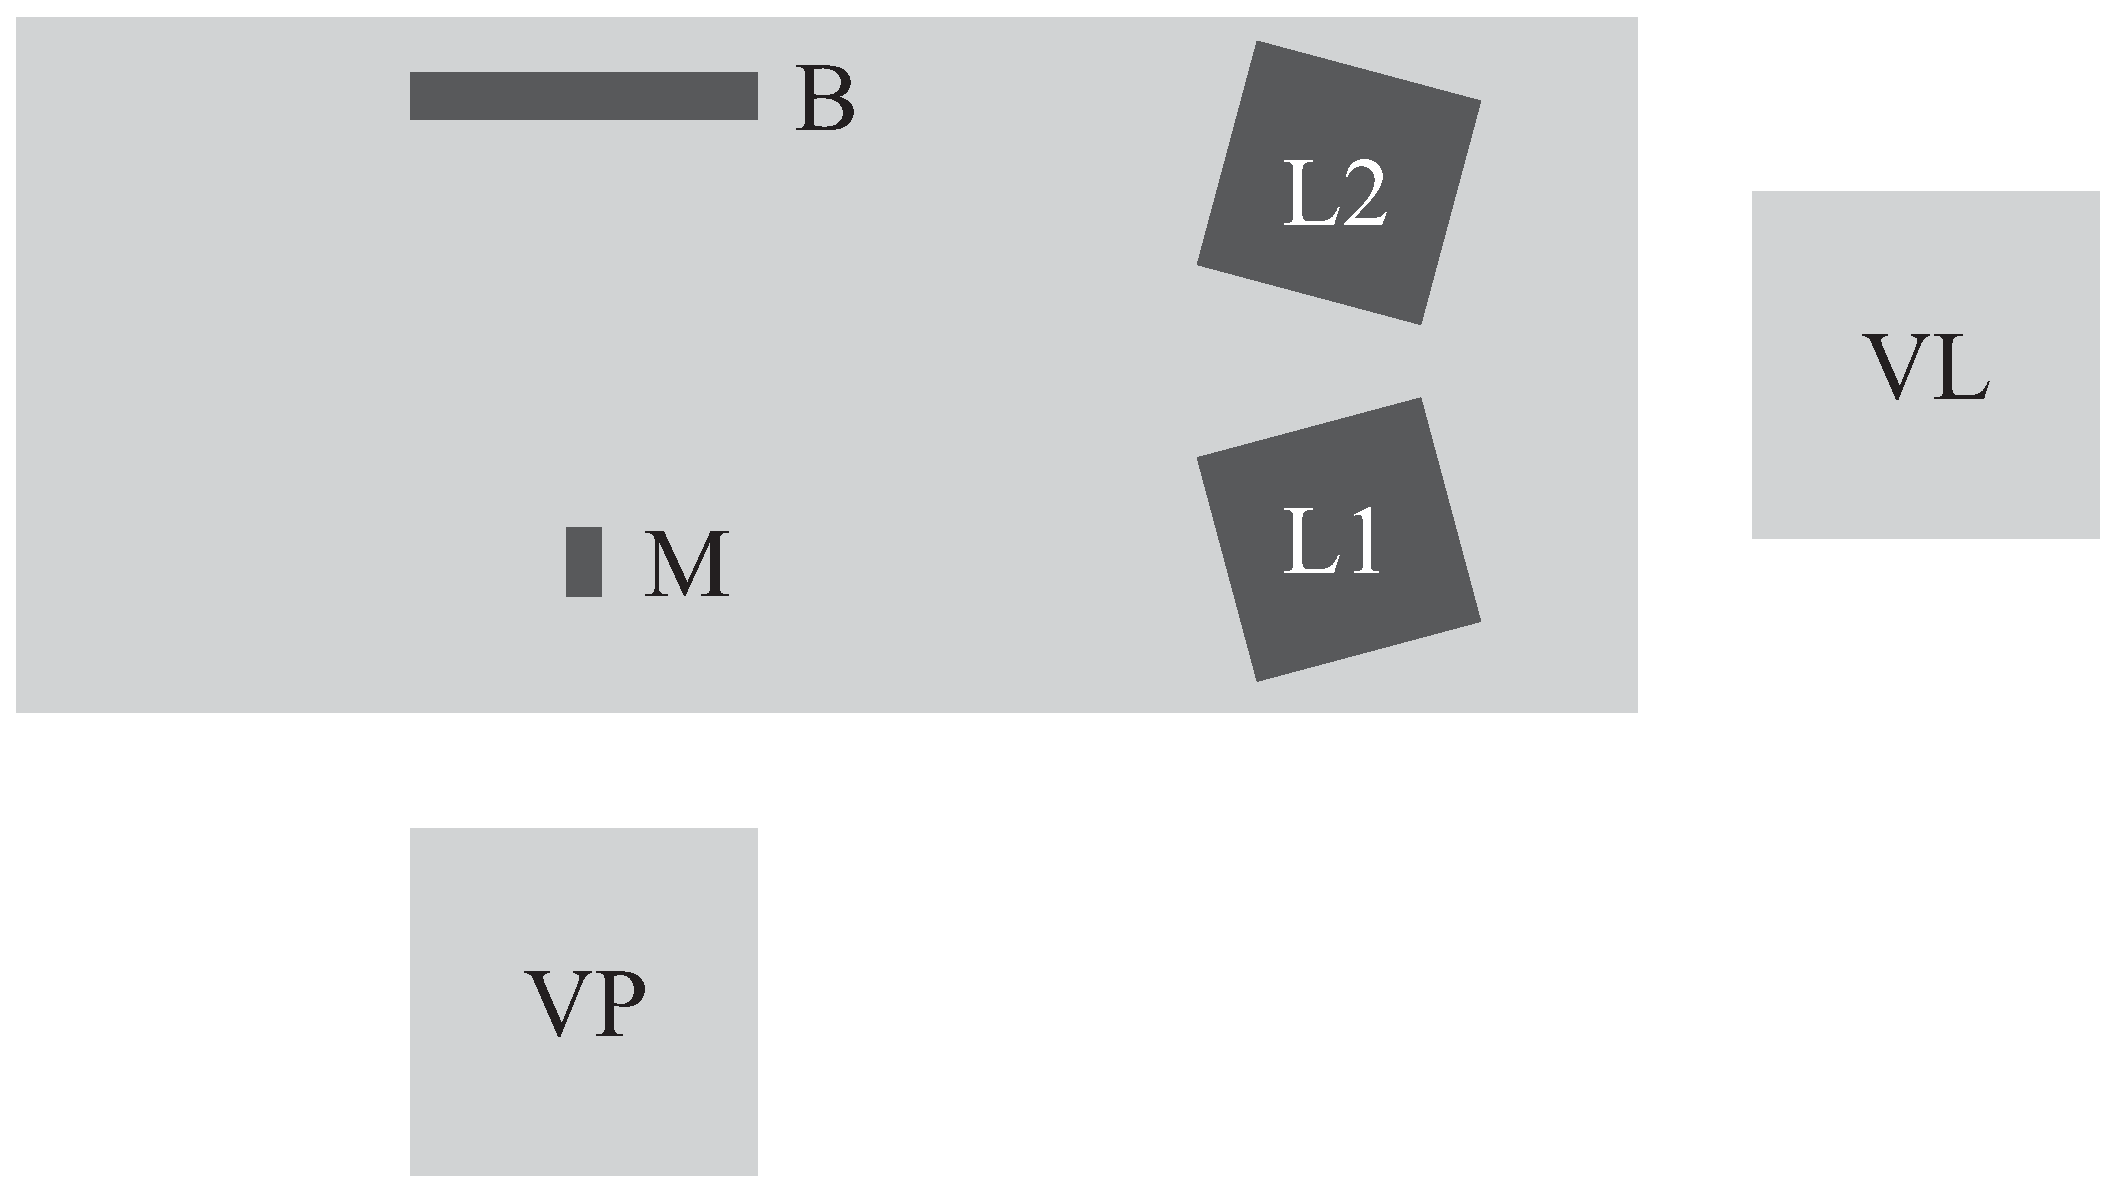
\includegraphics[width=\textwidth]{abb1-versuchsaufbau.eps}
    \end{minipage}}
    \vspace{10pt}
    \caption{Aufbau des Experimentes. Laptop 1 (L1) mit Programm für Experiment und Laptop 2 (L2) für Experimentator (E). Bildschirm (B), Maus (M) und Kopfhörer (nicht eingezeichnet) für Versuchsperson (VP).}
    \label{experiment}
  \end{minipage}
% ################
% Anhang ergänzen!
% ################
\end{wrapfigure}

Auf Laptop 1 (L1) wurde das Programm für den Versuch ausgeführt, dieser wurde vom Experimentator (E) bedient. Für das Abspielen der Töne und das Speichern der Reaktionsdaten wurde Matlab verwendet \footnote{\label{foot:1}Der Programmcode für den Versuch wurde in einer Vorversion von Prof. Dr. Alexandra Bendixen zur Verfügung gestellt.}. Der Laptop (L1) war an den Bildschirm (B) angeschlossen, welcher der Versuchsperson (VP) zur Verfügung stand. Auf diesem Bildschirm wurde angezeigt, wenn die Versuchsperson reagieren sollte. Zur Reaktion stand der Versuchsperson eine Computer-Maus (M) mit 2 Tasten zur Verfügung. Während in den bisherigen Experimenten auch immer eine EEG-Messung durchgeführt wurde, beschränkte sich dieses Experiment auf Reaktionsdaten (d-prime und Reaktionszeit). Des Weiteren wurde ein zweiter Laptop (L2) verwendet. Dieser wurde verwendet, damit sich Experimentator (E) während den Blöcken ablenken konnte. Unter Experimentalbedingungen im Labor sind Experimentator und Versuchsperson räumlich getrennt. In diesem Fall war eine räumliche Trennung nicht möglich. Um etwaige Versuchsleitereffekte zu minimieren, sollte der Experimentator nicht den Eindruck vermitteln die Versuchsperson zu beobachten oder gar zu kontrollieren. Auch subtile Reaktionen des Experimentators auf eventuelles gutes oder schlechtes Abschneiden der Versuchsperson sollten vermieden werden, indem der Experimentator von vorne herein den Bildschirm von L1 maximal abdunkelte und diesen nach Möglichkeit während der Stimulus-Präsentation nicht beachtete. Die Ablenkung an L2 erfolgte durch kognitiv anstrengende Aufgaben. Dabei wurde beachtet, dass der Experimentator nach dem Ende eines Blockes unverzüglich wieder zur Versuchsperson umschalten musste. Die Versuchsperson musste nach Beendigung eines Blockes ohne Unterbrechung direkt die volle Aufmerksamkeit bekommen, um die Motivation aufrecht zu erhalten.

Um Störungen von außen zu vermeiden wurde ein Schild an die Tür angebracht, welches darauf hinwiese, dass in diesem Raum ein Experiment am Laufen ist. Außerdem wurde das Fenster geschlossen und die Kopfhörer wurden vorher auf eine normierte Lautstärke eingestellt. Alle Utensilien (Maus, Kopfhörer, Formulare) wurden vorpräpariert auf den Tisch gelegt (bei Position M). Auch alle Einstellungen am Programm wurden vor der Ankunft der Versuchsperson vorbereitet, der Bildschirm (B) war zunächst ausgeschaltet und wurde erst unmittelbar vor dem Start des Versuchs eingeschaltet.

\subsection{Stimuli}

Innerhalb der Blöcke bekam die Versuchsperson auditive Stimuli präsentiert. Diese bestanden aus Tonsequenzen à 10, 15 oder 20 Tönen. Dabei waren die Töne und die Regel entsprechend denen bei Paavilainen et al. (2006). Die Töne unterschieden sich in Höhe (hoch/tief) und Länge (kurz/lang). Dabei wurden die Frequenzen für hohe (1500Hz) und tiefe (1000Hz) Töne wie zuvor verwendet. Auch die Länge der Töne blieb mit 50ms für Kurze und 150ms für lange Töne identisch zu den vorigen Experimenten. Die Regel für die Töne lautete wie zuvor bereits in der Einleitung beschrieben:

\begin{compactitem}
  \item Auf einen langen Ton folgt ein hoher Ton, auf einen kurzen Ton folgt ein tiefer
Ton
  \item Auf einen langen Ton folgt ein tiefer Ton, auf einen kurzen Ton folgt ein hoher
Ton
\end{compactitem}

Unterschiede zu den vorigen Experimenten gab es beim Inter-Stimulus-Intervall (ISI), welches zwischen den Blöcken variierte. Angewendet wurden Intervalle von 300ms, 600ms und 900ms. Der letzte Ton in 50\% der Fälle eine Ausnahme und wich von der gegeben Regel ab. Dabei wurden die Sequenzen nicht kontinuierlich präsentiert. Die nächste Sequenz startete erst, sobald ein Tastendruck ausgeführt wurde, hierfür hatten die Probanden beliebig viel Zeit, wurden jedoch angehalten relativ zügig zu reagieren. In Abbildung \ref{stimuli} in der Einleitung ist eine Beispielsequenz mit einer Abweichung am Ende skizziert.\\
Die Versuchsperson sollte mit der Maus nun darauf reagieren und entscheiden, ob der der letzte Ton passend oder abweichend ist. Dem zufolge liegt die Leistung der Versuchsperson darin zunächst die Regel zu erkennen, die letzten, zuletzt gespielten Töne im Gedächtnis zu behalten und nach Beendigung er Sequenz eine Entscheidung zu treffen. Auf dem Bildschirm war während den Sequenzen ein Fixationskreuz zu sehen, welches unmittelbar nach dem letzten Ton der Sequenz in ein Fragezeichen wechselte. Da die Sequenzen unterschiedlich lang waren, sollte dieses Hilfsmittel die Unsicherheitszeit zwischen den Sequenzen, die mindestens dem Inter-Stimulus-Intervall entspricht, möglichst gering zu halten. Eine systematische Reaktionszeit-Variation zwischen den Blöcken sollte damit vermieden werden.

\subsection{Ablauf}

Der Ablauf des Experimentes erfolgte nach einer standardisierten Checkliste. Damit konnte der Experimentator überprüfen, ob nach jedem Schritt alle relevanten Punkte erläutert wurden. Die Liste war für die Versuchsperson nicht sichtbar. Folgender Ablauf wurde durchgeführt:

\begin{compactenum}
  \item \textbf{Vorbereitung}: Präparation des Versuchsraumes (vor dem Eintreffen der VP)
  \item \textbf{Einführung}: Erklärung des Experimentes
  \item \textbf{Block 1 (schnell)}: Durchgang mit ISI von 300ms
  \item \textbf{Arbeitsblatt}: Lernen der Regel mit Hilfe eines Arbeitsblattes
  \item \textbf{Block 2 (langsam)}: Durchgang mit ISI von 900ms und Feedback
  \item \textbf{Block 3 (mittel)}: Durchgang mit ISI von 600ms und Feedback
  \item \textbf{Block 4 (schnell)}: Durchgang mit ISI von 300ms
  \item \textbf{Nachbereitung}: Musikfragebogen, Datensicherung
\end{compactenum}

Die Variation der ISI zwischen den Blöcken ist, ebenso wie das Arbeitsblatt, ein Lernprozess im Sinne der Lerntheorie von \textcite{fitts1967human}. Dabei repräsentiert das Arbeitsblatt das kognitive Stadium mit einem Übergang in das assoziative Stadium. Block 2 und Block 3 bilden das assoziative Stadium und sollten im Idealfall in Block 4 in das autonome Stadium überführen.

\subsubsection{(1) Vorbereitung}

In der Vorbereitung wurde kontrolliert, dass das Mobiltelefon auf stumm geschaltet ist, die Lautstärke (Windows 7 Betriebssystem) - falls noch nich geschehen - auf 40 eingestellt und der Laptop-Bildschirm abgedunkelt. Außerdem wurde das Fenster geschlossen (sofern vorher gelüftet wurde), Formulare und Stift, sowie Kopfhörer und Maus wurden bereitgelegt. Letztlich wurden einige Minuten für einen Moment der Ruhe eingeplant um konzentriert, klar und ruhig mit der folgenden Versuchsperson umgehen zu können.

\subsubsection{(2) Einführung}

Nach dem Unterschreiben der Formulare wurden die Rahmenbedingungen des Experimentes erklärt. Dabei wurde beim ersten Durchgang noch nicht die Regel erklärt. Der erste Durchgang diente als Kontrolldurchgang. Der Versuchsperson wurden folgende Fakten erklärt:

\begin{compactitem}
\item Eine Sequenz besteht aus 10-20 Tönen
\item Ein Block besteht aus 24 Sequenzen
\item Die Töne unterscheiden sich in Höhe (hoch/tief) und Länge (kurz/lang)
\item Der letzte Ton einer Sequenz kann zu den vorigen passen oder nicht passen
\item Eine Maustaste für "passt", eine für "passt nicht"
\item Erster Durchgang wird intuitiv gelöst
\end{compactitem}

Ergänzend erklärt wurde außerdem, dass der Experimentator während den Blöcken keine Ergebnisse beobachtet und sich an Laptop 2 ablenken wird. Außerdem wurde der Versuchsperson verdeutlicht, dass Genauigkeit wichtig ist. Letztlich bekam die Versuchsperson noch eine Empfehlung zur Bedienung der Maus. Die Tastenbelegung der Maus variierte zwischen den Versuchspersonen gleichmäßig, um eventuelle Effekte von Händigkeit auszuschließen. Die Versuchsperson bekam die Tastenbelegung vor jedem Block auf einem Startbildschirm angezeigt.

\subsubsection{(3) Block 1}

In Block 1 wurde zunächst ein Inter-Stimulus-Intervall von 300ms verwendet. Dies entspricht dem ISI von \textcite{paavilainen2007preattentive} und \textcite{bendixen2008rapid}. Nach dem der erste Block beendet war, wurde die Versuchsperson gefragt, ob sie eine Regel erkannt hatte. Sofern die Versuchsperson dies verneinte oder keine korrekte Regel nannte, wurde die Versuchsperson durch den Experimentator ermutigt mit der Aussage, dass noch niemand jemals zu diesem Zeitpunkt eine Regel erkannt habe und das Nicht-Erkennen der Regel ein wichtiger Bestandteil des Experimentes sei.

\subsubsection{(4) Arbeitsblatt}

In diesem Schritt, unmittelbar nach Block 1, wurde der Versuchsperson ein Arbeitsblatt (siehe Anhang) gegeben. Dafür setze sich der Experimentator neben die Versuchsperson an die lange Kante des Tisches neben Position VP. Das Arbeitsblatt wurde in allen Fällen gemeinsam bearbeitet. Dabei wurde zunächst anschaulich die Regel erklärt. Anschließend war die Versuchsperson aufgefordert für beide Regeln je eine eigene Sequenz zu erfinden und zu zeichnen. Bis zu diesem Punkt handelte es sich noch um die kognitive Stufe. Auf der letzten Seite des Arbeitsblattes wurde dann in die assoziative Stufe gewechselt. Dort waren Sequenzen vorgegeben, bei denen bestimmt werden musste, ob der letzte Ton regelkonform oder abweichend ist. Diese Übung entsprach in visuell/bildlicher Form der auditiven Übung und sollten der Festigung der verstandenen Regel dienen. Nach Beendigung des Arbeitsblattes wurde dieses für die Versuchsperson unzugänglich abgelegt, um gleiche Bedingungen für alle Versuchspersonen zu schaffen und eine Zuhilfenahme der Arbeitsblatt-Unterlagen generell auszuschließen. Im Anschluss wurde der Versuchsperson das weitere Vorgehen erläutert. Dabei wurde die Versuchsperson explizit darauf vorbereitet, dass die Regelerkennung bzw. das Erkennen eines Abweichers im auditiven Experiment deutlich schwieriger ist, als auf dem Blatt, um die Motivation möglichst hoch zu halten.

\subsubsection{(5) Block 2}

Block 2 erfolgte mit einem ISI von 900ms. Block 2 ist damit der langsamste Block und sollte einen guten Übergang von der Arbeitsblatt-Übung zu der auditiven Übung ermöglichen. Zur Unterstützung des Lernens wurde nach jedem Tastendruck ein kurzes Feedback angezeigt, ob die Sequenz richtig oder falsch beurteilt wurde. Nach Block 2 wurde die Versuchsperson kurz offen befragt (z.B. "Wie war es?"). Relevante Antworten wurden notiert. Der Versuchsperson wurde ein kurze Pause angeboten.

\subsubsection{(6) Block 3}

Block 3 erfolgte analog zu Block 2, jedoch mit einem ISI von 600ms. Block 3 sollte das Gelernte weiter festigen.

\subsubsection{(7) Block 4}

In Block 4 wurde das ISI wieder auf die ursprünglichen 300ms gestellt. Das Feedback wurde in diesem Block nicht mehr angewendet, da an diesem Punkt davon ausgegangen wird, dass die Versuchsperson bereits das autonome Stadium erreicht hat.

\subsubsection{(8) Nachbereitung}

Nach Block 4 wurde die Versuchsperson ein letztes Mal offen über den Versuch befragt. Zuletzt wurden letzte Formalien geklärt und ein Fragebogen zur Musikalität ausgefüllt. Nach dem Verlassen der Versuchsperson wurden alle Daten gesichert, bei Bedarf gelüftet und die nächste Vorbereitung eingeleitet.

Die Hypothese, die in der Einleitung formuliert wurde, lässt sich an dieser Stelle anhand des Experimentes präzisieren. Wenn ein expliziter Lernprozess prozeduralen Wissens nach der Lerntheorie möglich ist, dann sollte Block 4 signifikant von Block 1 bzw. vom Zufall abweichen.

\section{Ergebnisse}

Auch in diesem Experiment hatten zwar ein paar Versuchspersonen eine Regel erkannt. Meist konnte diese aber nicht gut konkretisiert werden. Die erkannten Regeln entsprachen in keinem Fall der tatsächlichen Regel.\\
Nach der Erläuterung der Regel (Schritt 4) verstanden alle Versuchspersonen die Aufgabe und konnten die letzten Übungen immer selbstständig lösen. Sehr oft wurde dann im Verlauf des Experimentes berichtet, dass das Arbeitsblatt zwar das Verständnis ermöglicht hat, das Lösen der auditiven Übung jedoch trotzdem sehr schwer ist.

\begin{figure}[t]
  \centering
  \begin{minipage}{\textwidth}
    \fbox{\begin{minipage}{\textwidth}
      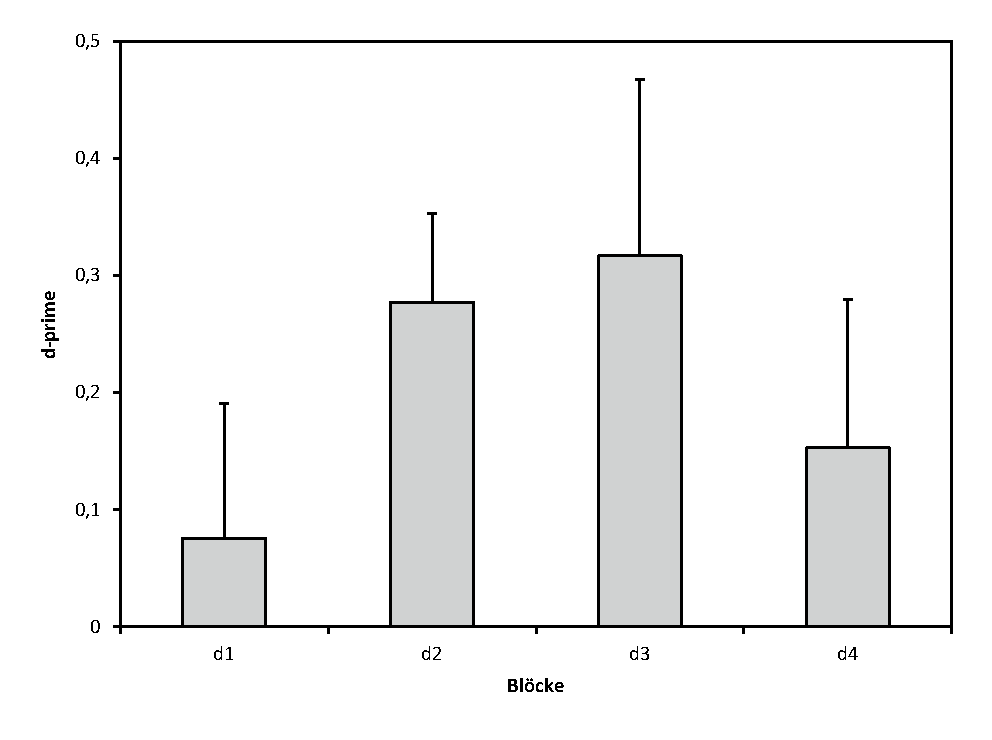
\includegraphics[width=\textwidth]{abb3-dprime.eps}
    \end{minipage}}
    \vspace{10pt}
    \caption{Mittelwerte der Sensitivitätsindizes über alle 18 Versuchspersonen in den Blöcken 1 - 4 mit Standardfehler}
    \label{dprime}
  \end{minipage}
\end{figure}

Die Richtig-Positiv-Rate (hit rate) lag in Block 1 bei 40.74\%, die Falsch-Negativ-Rate (false alarm rate) bei 37.04\%. In Block 4 lag die Richtig-Positiv-Rate dann bei 41.67\%, die Falsch-Negativ-Rate bei 35.65\%. In Abbildung \ref{dprime} ist der Sensitivitätsindex (d-prime) der 4 Blöcke abgebildet. Von Bedeutung ist an dieser Stelle der d-prime der Blöcke 1 und 4, Blöcke 2 und 3 dienten lediglich zur Übung.  Blöcke 1 und 4 waren beide mit einem ISI von 300ms und beide ohne Feedback. Der erste Block wurde ohne das Regelwissen durchgeführt, der vierte Block nach Vermittlung des Wissens über die Regel und nach Übung der Regel. Der Sensitivitätsindex in Block 1 beträgt d = 0.076 (SE = 0.115), in Block 4 liegt er bei d = 0.153 (SE = 0.126). Beide Werte unterscheiden sich nicht signifikant, t(17) = 0.56, p > 0.05. Auch wenn Block 4 gegen Null getestet wird, liegt der Sensitivitätsindex von Block 4 nicht signifikant über dem Zufallsniveau, t(17) = 1.22, p > 0.05.

%ROC-Kurven - Wie macht man das??

\section{Diskussion}

Da sich der Sensitivitätsindex in Block 1 und Block 4 nicht unterscheiden, sprechen die Ergebnisse gegen einen Lerneffekt. Die qualitative Auswertung der Berichte der Versuchspersonen passen gut zu den Ergebnissen, denn auch die Versuchspersonen berichteten - vor allem im letzten Durchgang - relativ konsistent von großen Schwierigkeiten beim Detektieren von Passenden und Abweichern am Ende der Sequenzen. Sie gaben an meist intuitiv entschieden zu haben und vor allem in den schnellere Durchgängen oft auch einfach nur geraten zu haben.

Dies lässt zwei mögliche Schlussfolgerungen zu. Zum einen könnte dieser Typ von Aufgabe zu komplexe sein, um ihn manuell und bewusst verarbeiten zu können. Die menschlichen Fähigkeiten wären in diesem Fall an ihren Grenzen. Zum anderen könnte aber auch der Lernprozess noch nicht ausreichend gestaltet worden sein. Bei der Gestaltung des Lernprozesses gibt es gleich mehrere Aspekte, die betrachtet werden müssen. Möglich wäre, dass die Zone proximaler Entwicklung nicht optimal gestaltet wurde. Die Lernmethodik wäre also auf Grund der hohen Komplexität immer noch zu schnell. Eine andere Option wäre, dass die Lernmodelle nicht auf die Aufgabe passen. Entweder sind die Modelle nicht für das Lernen hoch komplexer Regeln ausgelegt oder die Klassifikation des Lernprozesses in prozedurales Wissen war eine zu starke Vereinfachung. Um diese Optionen evaluieren zu können wurden im folgenden Kapitel "Post-Hoc Analysen" einige weitere statistische Analysen durchgeführt, die über die eigentliche Hypothese hinausgehen, aber eventuell Hinweise liefern können, die bei der Gestaltung zukünftiger Experimente helfen können. Ziel sollte es nun zum einen die vorliegende Prozesse präziser zu klassifizieren und zum anderen eine Systematik zur weiteren Untersuchung zu entwickeln.

\subsection{Sensorische Verarbeitung}

Die Ergebnisse stützen die Annahme von \textcite{paavilainen2007preattentive} und \textcite{bendixen2008rapid}, dass der Erkennungsprozess, der die MMN auslöst, im auditiven sensorischen Gedächtnis präattentiv abläuft. Weder ein expliziter, noch ein impliziter Lernerfolg konnte festgestellt werden, womit das Wirken höherer kognitiver Bereiche an dieser Stelle nicht anzunehmen ist. Unter der Annahme, dass die MMN - auch wenn sie hier nicht erfasst wurde - vermutlich auch in diesem Experiment aufgetreten ist, kann geschlossen werden, dass nur sensorische Prozesse eine Erkennung ermöglichen können.

\subsection{Lernbedingungen und Lernmethodik}

Offen bleibt an dieser Stelle, ob ein Lernprozess eventuell unter besseren Lernbedingungen funktioniert hätte. Wie oben schon angesprochen gibt es viele denkbare Möglichkeiten warum der Lernprozess eventuell nicht erfolgreich war. Entsprechend können an dieser Stelle einige Optimierungsansätze formuliert werden.

\subsubsection{Lernbedingungen}

Die Untersuchungsbedingungen verliefen in keinem schalldichten Raum, sondern unter eher provisorischen Bedingungen in einem für das Experiment präparierten Raum. Auch wenn Tür und Fenster immer geschlossen blieben, waren Geräusche von außen nicht gänzlich zu verhindern. Auch die Tatsache der direkten Anwesenheit des Experimentators könnte, trotz der angewendeten Ablenkungsstrategie, einen negativen Effekt auf die Versuchspersonen gehabt haben. Allein eine kleine Bewegung - sei es nur eine Veränderung der Sitzposition - könnte durch die Nähe schon eine Ablenkung bedeuten, zumal die Konzentrationsanforderungen bei dem Experiment für die Versuchspersonen enorm hoch war. Unter optimalen Bedingungen sind Versuchsperson und Experimentator während den Blöcken räumlich getrennt.

\subsubsection{Lernmethodik}

Ein anderer wichtiger Aspekt ist die Verbesserung der Lernmethodik. Der Lernaufwand wurde stark unterschätzt und der Lernprozess sollte deutlich umfassender gestaltet werden. Dazu könnten zum Beispiel weitere langsame Blöcke eingefügt werden. Etwas ungünstig war ohnehin, dass es keine Übung mit Feedback für den vierten Block hab. Nach konsequenter Einhaltung der Lerntheorie hätte auch Block 4 noch einmal geübt werden müssen, bevor davon ausgegangen werden kann, dass dieser automatisiert ausgeführt werden kann. Genau genommen könnte davon ausgegangen werden, dass die Testdurchführung von Block 4 noch im assoziativen Stadium durchgeführt wurde und das autonome Stadium noch gar nicht möglich war. Diese Vermutung geht direkt mit der bereits oben genannten Annahme einher, dass die Zone proximaler Entwicklung nicht optimal angewendet wurde. Grundsätzlich ist jedoch - nicht zuletzt auch aufgrund der qualitativen Beurteilung - davon auszugehen, dass ein einfaches Einfügen eines weiteren schnellen Übungsblockes zu keiner nennenswerten Leistungssteigerung führen dürfte. Ein erfolgsversprechender Lernansatz müsste die Lernmethode deutlich erweitern. Eventuell müssten auch Lerneffekte durch Pausen und Schlaf berücksichtigt werden, was den Lernprozess über mehrere Tage hinziehen könnte, bis eine Leistung mit deutlich erhöhter Sensitivität erreicht wird. Ein weitere Aspekt ist die nötige Trennung des Lernprozesses in seine kognitiven Bestandteile. Bei der auditiven Übung mussten zwei Leistungen erbracht werden. Zum einen musste die Regel möglichst schnell erkannt werden (Erkennungsleistung), zum anderen mussten die letzten zwei Töne im Gedächtnis behalten werden (Gedächtnisleistung). Auf dem Arbeitsblatt war immer die gesamte Sequenz zu sehen (siehe Anhang). Daher wurde dort lediglich die Erkennungsleistung geübt. Eine Versuchsperson berichtete zum Beispiel, dass das Hauptproblem für sie daran bestand die letzten Töne differenziert im Gedächtnis zu behalten. Es könnte dafür eine weitere Aufgabe gestaltet werden, in der zum Beispiel eine auditive Übung durchgeführt wird, in der es ausschließlich auf die Gedächtnisleistung ankommt. Beide kognitiven Bestandteile müssten von vorne herein klar mit der Versuchsperson kommuniziert und letztlich auch trainiert werden. Vorstellbar wäre, dass diese Übung in Kombination mit mehr Blöcken und dem Anwenden von Pausen zu passenden Zeitpunkten zu einer deutlichen Leistungssteigerung führen könnten. Letztlich sollte auch nach jedem Block strukturiert erfragt werden wie stark die Person subjektiv das Gefühl hatte geraten, intuitiv vermutet oder tatsächlich kognitiv versucht hat den letzten Ton zuzuordnen.

All diese Annahmen und Beobachtungen zeigen jedoch deutlich, dass die Lernmethodik beträchtlich verbessert werden muss und die Fähigkeiten für implizites, vor allem aber für explizites Lernen komplexer auditiver Regeln in der Vorbereitung dieses Experimentes noch erheblich unterschätzt wurden.

\section{Post-Hoc-Analysen}

Zusätzlich zu den Hypothesen-relevanten Informationen wurden einige weitere Daten erhoben. So liegen Daten über die Sensitivitätswerte von Block 2 und 3 vor, wie sie auch in Abbildung \ref{dprime} bereits dargestellt sind. Des Weiteren wurden bisher die Reaktionszeiten nicht betrachtet und letztlich wurde am Ende des Experimentes (siehe Methoden) ein Musikfragebogen durch die Versuchspersonen ausgefüllt, dessen Daten bisher auch noch nicht in der Analyse berücksichtigt wurde.

\subsection{Effekte in den langsamen Blöcken}

Um zu überprüfen, ob eventuell doch Lerneffekte vorliegen, diese nur nicht hinreichend für Block 4 waren, werden nun auch die Sensitivitätsindizes von Block 2 und 3 mit Block 1 und dem Zufall (Null) statistisch mit Hilfe eines T-Tests überprüft. Um die Alphafehler-Kumulierung zu berücksichtigen, wurde $\alpha$ halbiert, da zwei Blöcke getestet wurden. Die Die gerichtete Hypothese lautet, dass Block 2 und 3 durch Lerneffekte signifikant höher sind, als Block 1 bzw. als Null.

Bei der statistischen Prüfung zeigt sich zunächst, dass sich Block 2 nicht signifikant von Block 1 unterscheiden, t(17) = 1.69, p > 0.05. Das gleiche gilt für den Vergleich von Block 3 und Block 1, t(17) = 1.62, p > 0.05. Sie unterscheiden sich jedoch beide signifikant von Null, also dem Zufallsniveau. Für den Test von Block 2 gegen Null ergab sich ein T-Wert von t(17) = 3.64 (p < 0.01), für Block 3 gegen Null lag der T-Wert bei t(17) = 2.11 (p < 0.1) und war damit noch marginal signifikant.

Die Ergebnisse geben einen Hinweis darauf, dass der Lernprozess zu schnell stattfand. Während in Block 2 der Unterschied zum Zufall noch hochsignifikant ist, ist der Unterschied zwischen Block 3 und Zufall nur noch marginal signifikant. Die Ergebnisse unterstützen den Ansatz, dass bei Verbesserung der Lernmethodik auch eine Erkennungsleistung möglich wäre, die deutlich über dem Zufallsniveau liegt.

%Erkenntnisgewinn geht an dieser Stelle nicht über Paavilainen/Bendixen hinaus! Bestätigung geringer Lerneffekte.

\subsection{Effekte unterschiedlicher Strategien}

Bei Betrachtung der Daten war auffällig, dass die Reaktionszeiten sehr variierten. Innerhalb der Versuchspersonen schienen die Reaktionszeiten jedoch relativ ähnlich zu sein. Diese Beobachtung lässt vermuten, dass die Versuchspersonen unterschiedliche Strategien anwendeten. Ließen sich die Versuchspersonen viel Zeit, so liegt das vermutlich an einer stark kognitiv orientierten Erkennungstrategie. Reagierten die Versuchspersonen relativ schnell, dann lässt das auf eine eher intuitive Verarbeitung schließen.

\begin{figure}[t]
  \centering
  \begin{minipage}{\textwidth}
    \fbox{\begin{minipage}{\textwidth}
      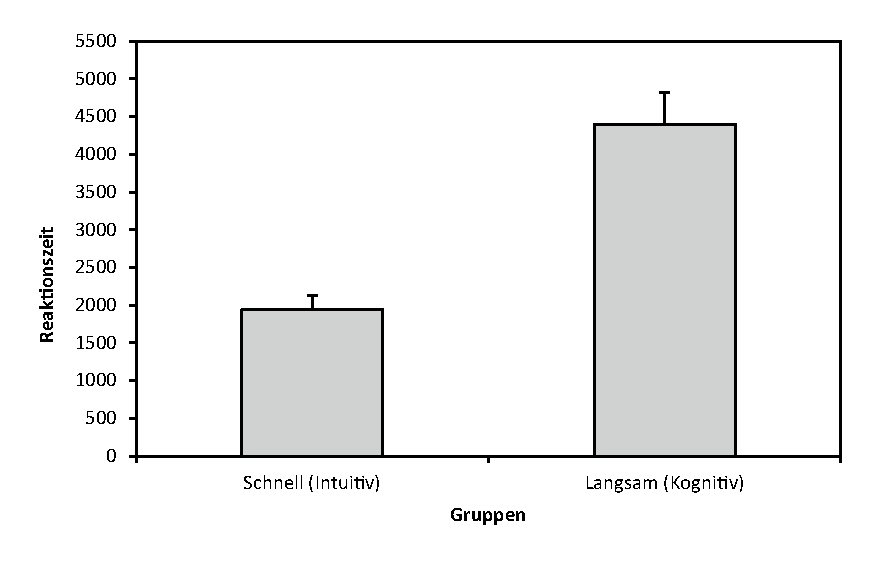
\includegraphics[width=\textwidth]{abb4-strategien.eps}
    \end{minipage}}
    \vspace{10pt}
    \caption{Mittelwerte und Standardfehler der Reaktionszeit der zwei Guppen mit je 9 Versuchspersonen. Die Gruppen wurden durch einen Mediansplit getrennt.}
    \label{strat}
  \end{minipage}
\end{figure}

Um diese Beobachtung statistisch zu prüfen wurden zunächst Mittelwerte der Reaktionszeiten jeder Versuchsperson über alle 4 Blöcke berechnet. Damit wurde jeder Versuchsperson eine mittlere Reaktionszeit zugeordnet. Anhand dieser Daten wurde ein Mediansplit vorgenommen. Mit Hilfe des Mediansplits konnte gezeigt werden, dass sich die Gruppe mit den höheren mittleren Reaktionszeiten (M = 4400 ms, SE = 414 ms) hochsignifikant von den der Gruppe mit den niedrigeren Reaktionszeiten (M = 1939 ms, SE = 194 ms) unterschied, t(11) = 15.38, p < 0.001. Die Mittelwerte und Standardfehler der Gruppen sind in Abbildung \ref{strat} dargestellt. Es scheinen also tatsächlich zwei unterschiedliche Strategien zur Erkennung angewendet worden zu sein. Interessanterweise war jedoch keine der Gruppen besser. Bei den Versuchspersonen mit der schnellen Strategie ergab sich kein Unterschied zwischen Block 4 und Block 1 im Sensitivitätsindex, t(8) = 1.66, p > 0.05 und kein Unterschied zwischen Block 4 und dem Zufall, t(8) = -0.23, p > 0.05. Das Gleiche ergab sich für die kognitive Strategie bei Block 4 und Block 1, t(8) = -0.6, p > 0.05 und bei Block 4 gegen Zufall, t(8) = 1.77, p > 0.05. Auch wenn die Leistungen der Versuchspersonen innerhalb von Block 4 verglichen wurden, ergab sich keine signifikant bessere Leistung eine der beiden Strategien, t(15) = -1.54, p > 0.05.

Es kann davon ausgegangen werden, dass tatsächlich eine eher intuitive (implizite) Strategie und eine eher kognitive (explizite) Strategie angewendet wurde. Gleichzeitig führte keine von beiden Strategien zu einem besseren Ergebnis. Dieses Ergebnis stützt die Annahme, dass ein Lernen der komplexen Regel nicht möglich ist, da selbst unter hohem kognitiven Aufwand keine signifikant besseren Ergebnisse erzielt wurden.

\subsection{Effekte von Musikalität}

...

%Fragen wie Musikfragebogen ausgewertet werden kann. Musikalitäts-Index?

\subsection{Möglicher Forschungsansatz}

Auf Basis der weitergehenden Analysen soll an dieser Stelle eine Begriffstrennung vorgenommen werden, die in der bisherigen Betrachtung nicht sauber unternommen wurde. Für zukünftige Experimente könnte diese begriffliche Einordnung aber von hoher Bedeutung sein. Für diese Klassifikation müssen zunächst einige Annahmen getroffen werden: (1) Erkennungsprozesse laufen kumulativ und automatisch auf sensorischer Ebene ab, (2) implizite Lerneffekte sind möglich - wie zumindest in den vorangegangenen Studien gezeigt wurde - und (3) explizite Lernprozess sind ebenfalls möglich. Ein Nachweis sollte  unter verbesserten Lernbedingungen und einer optimierten Lernmethodik möglich sein. Dies wird durch die Post-Hoc-Analyse von Block 2 und 3 gestützte, in denen ein kleiner Lerneffekt zu beobachten war. Werden die Annahmen vorausgesetzt, dann können die Lernprozesse neu eingeordnet werden. Dabei muss zunächst eine Korrektur in der Betrachtung der Lernprozesse vorgenommen werden. Bisher wurde getrennt zwischen manuell bewusst, in Form von explizitem Lernen, und automatisiert unbewusst, in Form von sensorischer Regelerkennung. Dabei ist eigentlich eher davon auszugehen, dass der manuell bewusste Lernprozess nur der Prozess ist, im Ergebnis jedoch ebenfalls zu einem Automatismus führt. Das autonome Stadium und die Unconscious competence entspricht eben diesem Automatismus. Implizite Lernprozesse führen ebenfalls zu einem Automatismus. Entscheidend ist, dass sich alle drei Mechanismen im Ergebnis ähnlich sein sollten. Der Weg zu dem jeweiligen Automatismus unterscheidet sich jedoch und bildet den entscheidenden Unterschied zwischen den drei Prozessen. Im Folgenden werden aus der genannten Folgerung vier Hypothesen aufgestellt:

\subsubsection{Hypothese 1}

Lernprozesse führen nach häufiger Übung der gleichen prozeduralen Einheit immer zu einer automatisierten Handlung. Dabei existiert neben dem impliziten und expliziten Lernen prozeduralen Wissens auch sensorisches Lernen.

\begin{compactitem}
  \item \textbf{Sensorisches Lernen}: Kumulativer Lernprozess durch Anhäufung von Hinweisreizen (Präattentive Verarbeitung)
  \item \textbf{Implizites Lernen}: Unbewusster Lernprozesse (Subattentive Verarbeitung)
  \item \textbf{Explizites Lernen}: Bewusster Lernprozess (Attentive Verarbeitung)
\end{compactitem}

\subsubsection{Hypothese 2}

Eine Beeinflussung impliziter und expliziter Prozesse erfolgt durch Achtsamkeit (mindfulness), wobei einmal eingeübte explizite Prozesse leichter zu verändern sind, als eingeübte implizite Prozesse. Eine Beeinflussung sensorischer Prozesse ist nicht möglich.

\subsubsection{Hypothese 3}

Sensorische Prozesse helfen Organismen bei der Bewältigung hochkomplexer Aufgaben. Implizite und explizite Prozesse sind weniger effektiv, jedoch adaptiv (Siehe Hypothese 2).

\subsubsection{Hypothese 4}

Die sensorische Ebene ist unabhängig von den anderen beiden Ebenen. Während implizite und explizite Automatismen voneinander profitieren können, arbeitet die sensorische Ebene isoliert.

Ob die 4 Hypothesen zutreffen oder nicht ist zunächst nicht zu klären und bisher philosophisch abgeleitet. Sie eignen sich jedoch recht gut um die Befunde erklären zu können. Daher könnte es interessant sein diese Hypothesen empirisch zu prüfen.

\subsection{Beispiele}

Sprache verstehen -> Implizites Lernen
Sprache Sprechen (Monitoring) -> Implizit/Explizit
Musik "fühlen" -> Sensorisches Lernen

%\subsection{Philosophische Betrachtung}

%Wenn die 4 Hypothesen zutreffen sollten, dann hätte dies nicht nur eine entscheidende Bedeutung für das Verstehen von Lernprozessen, es würde sich auch auf die in der Einleitung angesprochenen Themen anwenden lassen. Die Frage des freien Willens wäre dann eine Frage der Achtsamkeit - im Folgenden wird das Mindfulness-Konstrukt verwendet, beschrieben u.a. in \textcite{bishop2004mindfulness} - und somit keine automatisch gegebene menschliche Eigenschaft, sondern eine Fähigkeit, die man erlernen kann. Menschen mit einer hohen Ausprägung an Achtsamkeit wären demnach nicht nur in der Lage neue Automatismen gezielter zu lernen und zu verändern, sie können auch die sie steuernden Automatismen aus vergangenen Zeiten beeinflussen, zum Beispiel solche, die in der Kindheit erworben wurden. Diese Eigenschaft könnte eine der Hauptursachen für Resilienz ggü. psychischen Störungen sein. Dadurch, dass neue Automatismen effektiver gelernt werden können und adaptiver sind, dürfte diese Fähigkeit auch ein guter Prädiktor für Intelligenz sein, eventuell sogar ein basaleres Konzept darstellen.

%Aus dieser philosophischen Überlegung heraus, kann bei zukünftigen Studien auch untersucht werden, ob sich Achtsamkeit auf die explizite und/oder implizite Lernleistung der komplexen Regel auswirkt. Die hier genannte Überlegung würde nahelegen, dass Personen mit einer erhöhten Achtsamkeit beim Lernen der Regel eine bessere Leistung erbringen müssten.

\section{Zusammenfassung und Fazit}

Mit Sicherheit kann festgehalten werden, dass das Lernen einer komplexen Regel, wie sie hier angewendet wurde, sehr schwer ist, eventuell sogar unmöglich. Gleichzeitig kann festgehalten werden, dass das menschliche Gehirn einen Mechanismus auf sensorischer Ebene besitzt, der Regeln hocheffizient erkennen und Fehler detektieren kann. Dieser bleibt einem bewussten Zugang jedoch verwehrt. Folgende Studien müssten zunächst klären, ob ein explizites Lernen solcher Regeln überhaupt möglich ist. In der Diskussion wurden viele Optimierungsmöglichkeiten des Lernprozesses angesprochen. Sollte sich bewahrheiten, dass ein explizites Lernen nicht möglich ist, dann wäre eine Grenze der menschlichen Fähigkeiten bezüglich bewusster Verarbeitung gefunden. Sollte explizites Lernen entgegen den Befunden in diesem Experiment möglich sein, dann könnte im nächsten Schritt untersucht werden inwiefern sensorische und explizite Verarbeitung zusammenhängen. Dafür könnten zum Beispiel zwei Bedingungen verwendet werden, wobei in einer Bedingung lange Tonsequenzen mit einer Vielzahl an regelkonformen Tönen parallel zu einem Stummfilm gezeigt werden, in der anderen Bedingung würde dies nicht durchgeführt werden. In beiden Gruppen könnte dann ein funktionierendes explizites Lernverfahren angewendet werden und es würde sich zeigen, ob die Lernmechanismen voneinander profitieren können oder isoliert ablaufen.

Es kann an dieser Stelle festgehalten werden, dass sich die Prozesse in viele - teils sogar verwendete - Begriffssysteme nicht einordnen lässt. Die sensorische Verarbeitung kann nicht als implizit betrachtet werden, da Lerneffekte durch die sensorische Regelerkennung derzeit nicht nachgewiesen sind. Auf die Einordnung als prozedural oder deklarativ ist schwierig, da es keinen Bewegungsablauf gibt. Auch der Begriff einer unbewussten Verarbeitung ist nicht haltbar, da eine unterbewusste Verarbeitung immer noch nachhaltige Effekte auf das Verhalten aufweist, was hier nicht der Fall ist. Die einzige Möglichkeit den Begriff zu einzuordnen ermöglicht das Konzept der Aufmerksamkeit. Die Einordnung als präattentiv, also vor der Aufmerksamkeit ablaufend, ist die einzig präzise Einordnung. Ich persönlich bin der Ansicht, dass das Konzept der Aufmerksamkeit und vor allem das damit eng verknüpfte Konzept der Achtsamkeit (mindfulness) in der zukünftigen Forschung eine große Bedeutung haben wird (vgl. ...).

%Noch unsicher, ob wirklich rein nehmen

%Ob und inwiefern sich auch die philosophischen Betrachtungen bestätigen lassen sei an dieser Stelle offen gelassen, da eine fundierte empirische Grundlage für diese Betrachtung noch fehlt. Ein wichtiges Qualitätsmerkmal empirischer Forschung ist die Absicherung jedes noch so kleinen Schrittes, bevor weitreichende Theorien angenommen werden. Trotzdem sollten auch die philosophischen Fragestellungen nicht außer acht gelassen werden, denn sie sind es, die unser Verständnis von uns selbst, von unseren Fähigkeiten und Grenzen ansprechen und weitreichende Konsequenzen für unser Selbstverständnis, auch in Relation zu anderen Lebewesen, haben kann. Das menschliche Selbstverständnis hat eine Fülle weitreichender Konsequenzen für viele gesellschaftliche Entscheidungen und ethische Betrachtungen. Entsprechend ist auch die Formulierung gewagter Theorien ein wichtiger Schritt des Erkenntnisprozesse. Es ermöglicht die Fragestellungen zielgerichtete Forschungsfragen, bilden das Motiv für weitergehende Forschungen und gibt der Forschung einen direkten Sinn.

\section{Literaturverzeichnis}

\printbibliography[heading=none]

\end{document}